
\documentclass[PICOReport.tex]{subfiles}

\begin{document}

%Enumerate the various signals in polarization. Use the frequency band + signals figure. The challenge is to dig out the faintest of all signals, the one due to $r$. This sets the tone for the entire 'signal decomposition' or 'component separation'.  Removing the galactic signal to unmask $r \lesssim 0.001$ is a challenge for all future experiments searching for $r$ at that level, and is a strong advantage of a space platform. The physics of galactic signals suggests complexities in their combined emission properties; the level of this complexity is not known. } 

Diffuse Milky Way emissions dominate the sky's polarized intensity on the largest angular scales; see Figures~\ref{fig:clbb} and ~\ref{fig:pico-channels-and-fg}. Even though their levels decrease when considering smaller angular scales, they are still considerably brighter 
near the \ac{IGW} peak at $\ell=80$ when averaging over 60\% of the sky. 
Even in the cleanest, smaller patches of the sky, far from the galactic plane and thus relatively low in galactic emissions, their levels are expected to be substantial relative to the \ac{IGW} for $r \lesssim 0.01$, and dominate it for $r \lesssim0.001$. Separating the cosmological and Galactic emissions signal, also called foreground separation, together with control of systematic uncertainties are {\it the} challenges facing any next decade experiment attempting to reach these levels of constraints on $r$.

\begin{figure}
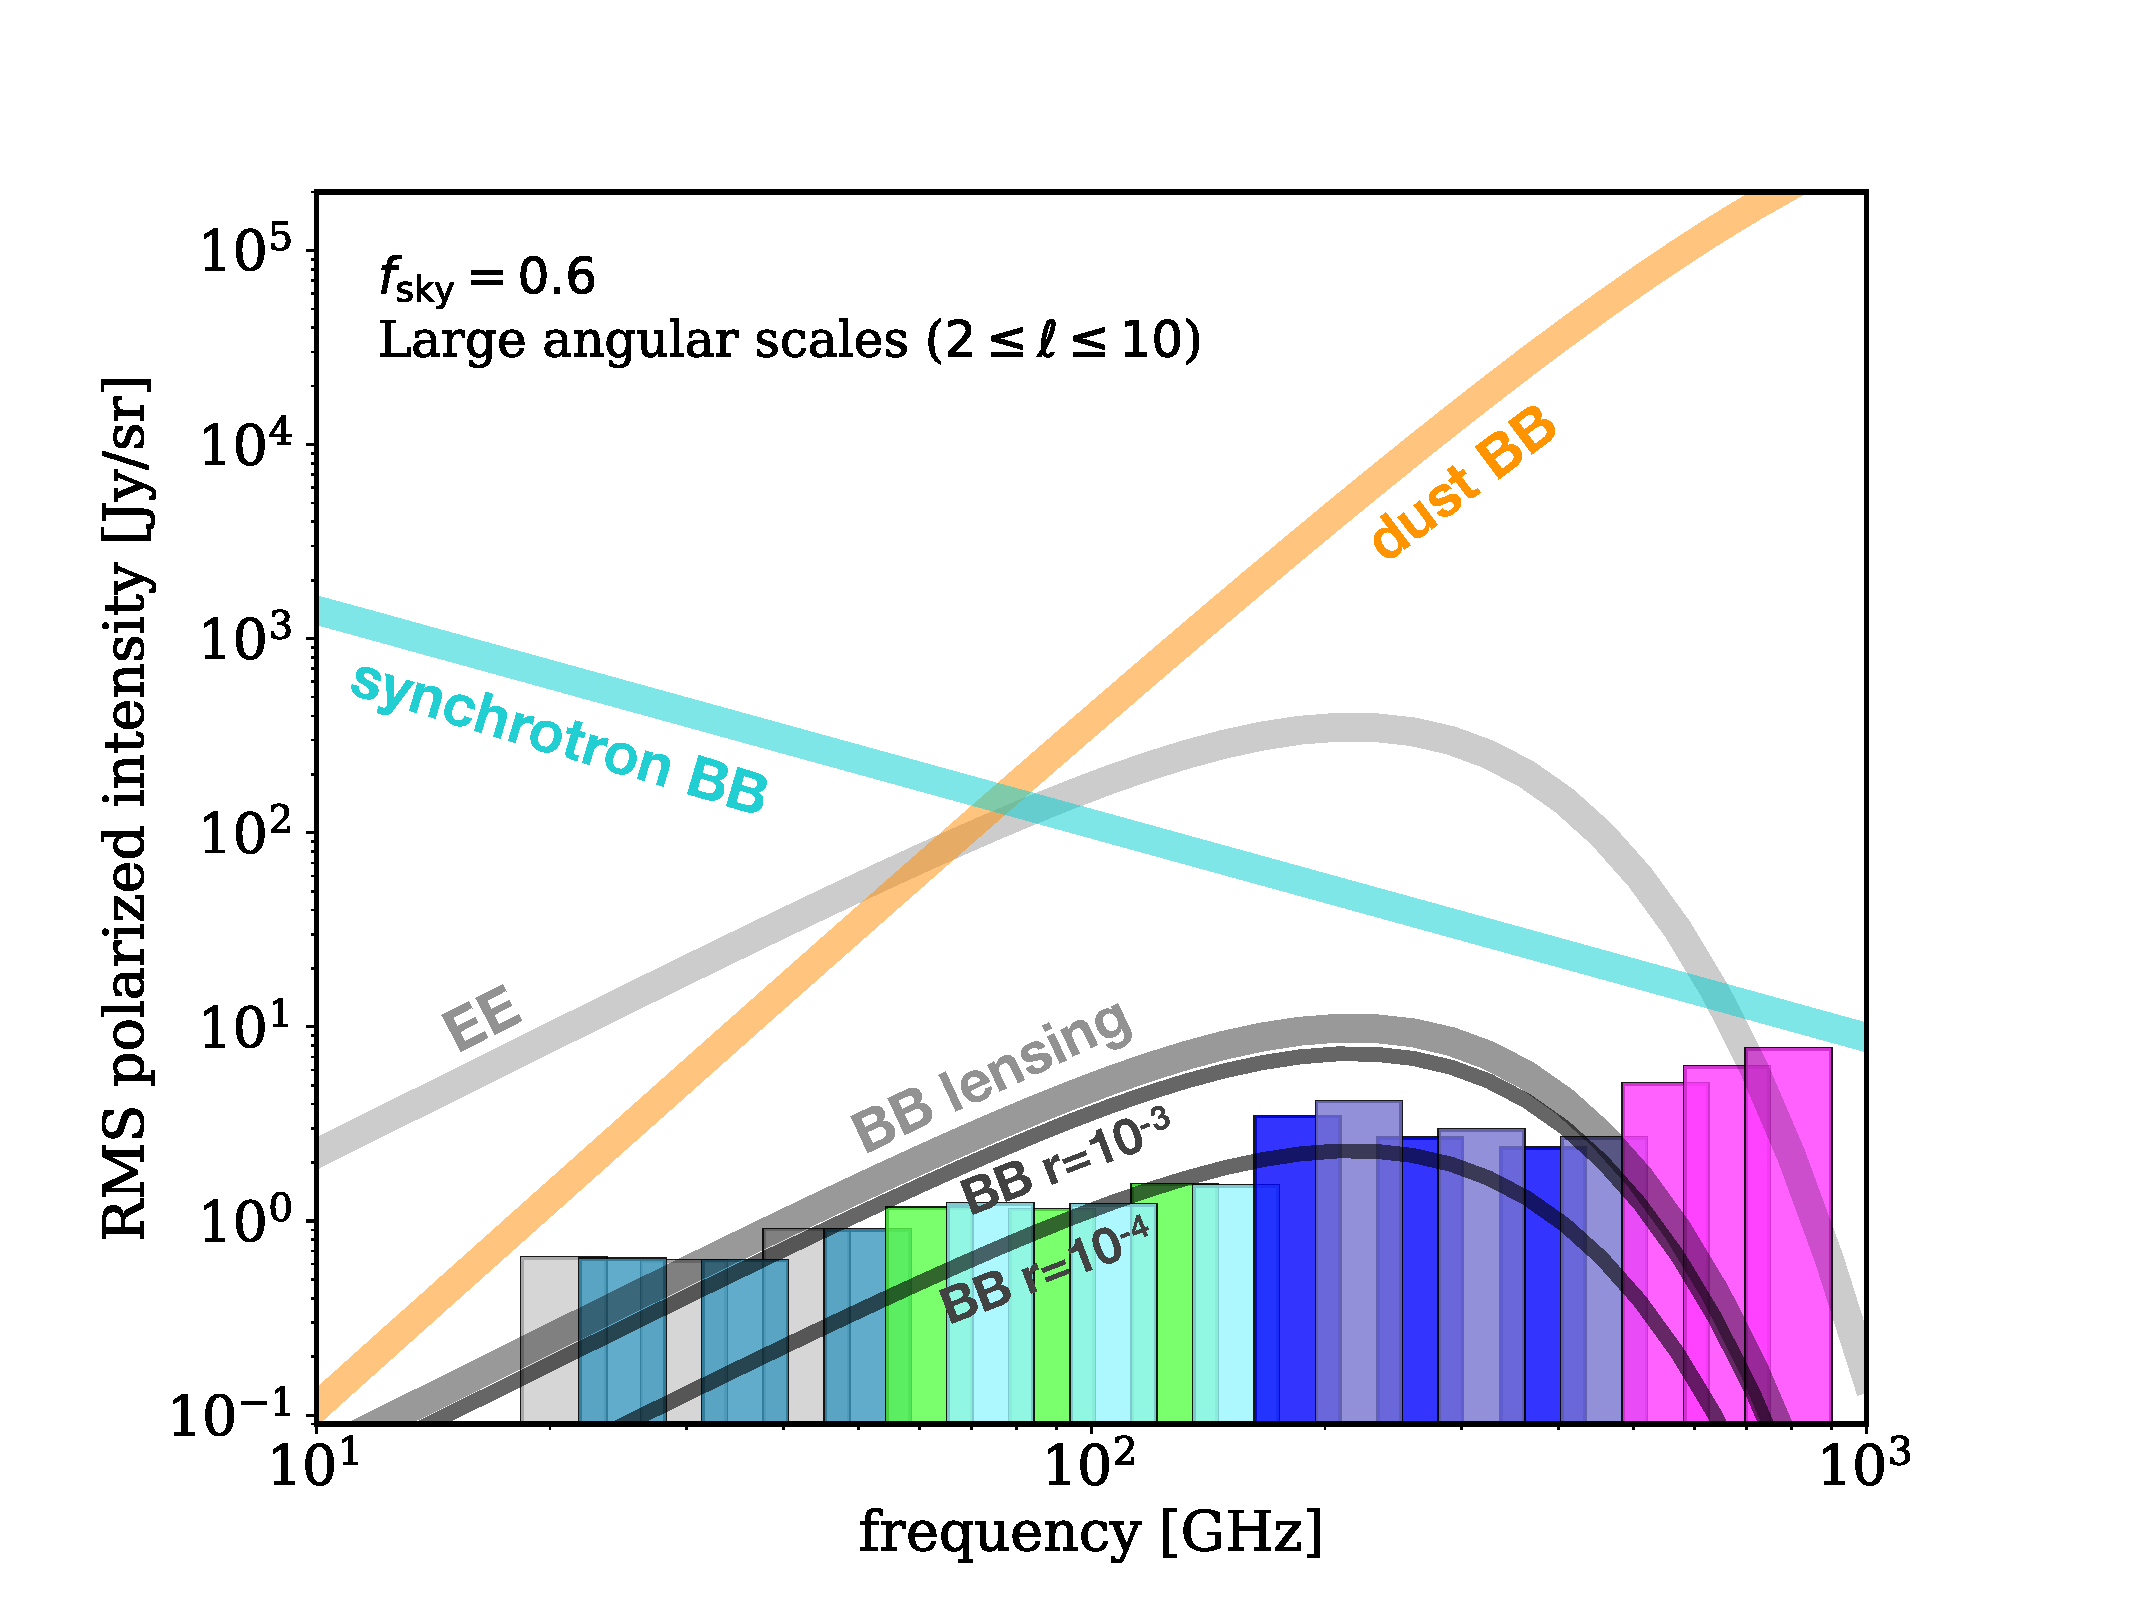
\includegraphics[width=0.49\textwidth]{images/sensitivity_vs_frequency_Jun29th_2018_large.pdf}
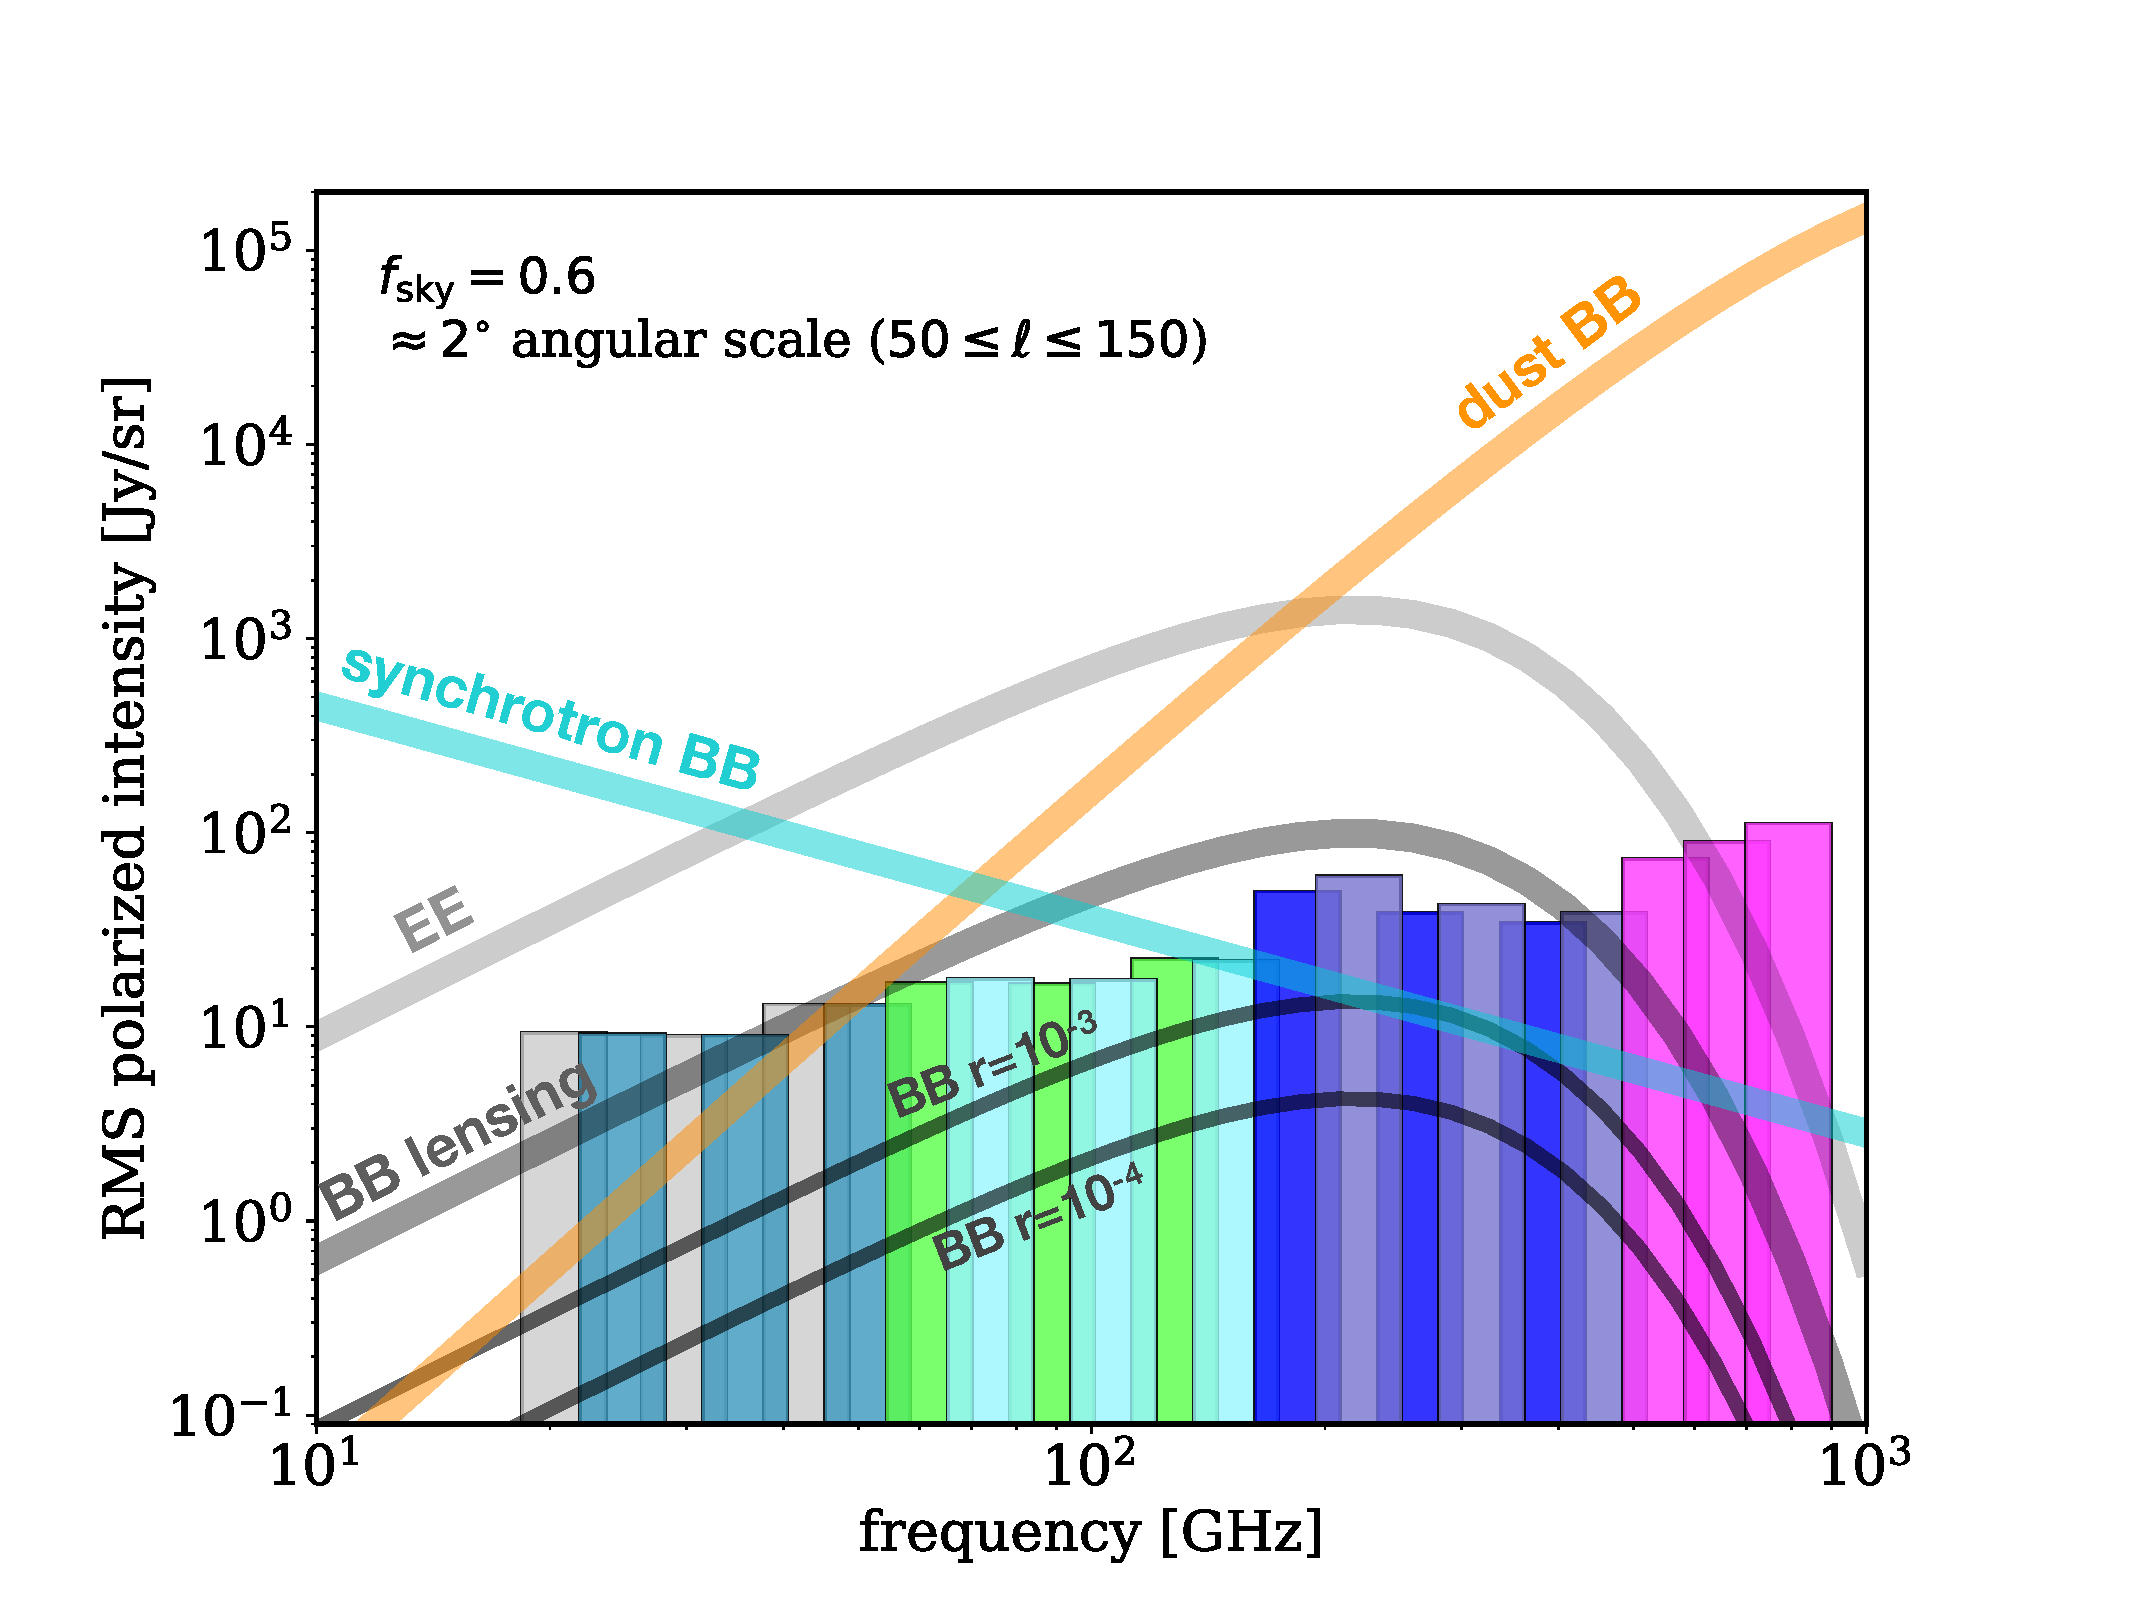
\includegraphics[width=0.49\textwidth]{images/sensitivity_vs_frequency_Jun29th_2018_2deg.pdf}
\vspace{-0.1in}
\caption{Polarization $BB$ spectra of Galactic synchrotron and dust, compared to CMB polarization $EE$ and $BB$ spectra of different origins for two values of $r$ and for two ranges of angular scales: large $\ell \leq 10$ corresponding to the reionization peak (left panel), and intermediate $50 \leq \ell \leq 150$ corresponding to the recombination peak (right panel). The location and sensitivity of the 21 PICO frequency channels is shown as vertical bands. (The color scheme is explained in Section~\comor{which? Karl}.) }
\label{fig:pico-channels-and-fg}
\end{figure}

The foreground separation challenge would be easily surmountable if the Galactic emissions were already precisely characterized, or were known to have simple, fittable spectral emission laws. But neither is true. Until recently, the spectrum of Galactic synchrotron emission, arising from free electrons spiraling around Galactic magnetic fields, was modeled as a power law $I_{\rm sync} \propto \nu^{\alpha},$ with $\alpha \simeq -1$ (in brightness units). The spectrum of Galactic dust emission, arising from emission by Galactic dust grains, was modeled as $I_{\rm dust} \propto \nu^{\beta} B_\nu(T_{\rm dust}),$ where $\beta \simeq 1.6$, $T_{\rm dust} \simeq 19$\,K, and $B_\nu(T)$ is the Planck function; this is referred to as `modified black body emission'. \comor{the values are averages across the sky?} In principle, an experiment that had 6 frequency bands could determine the three emission parameters as well as the three amplitudes corresponding to that of dust, synchrotron, and the CMB. However, WMAP and Planck observations have shown that neither emission law is universal and that spectral parameters vary with the region of sky \comor{is that true? is there evidence from Planck; add references} (thus that the values given above are valid only as averages across the sky). Also, while both emission laws are well-motivated phenomenological descriptions, the fundamental physics of emissions from grains of different materials, sizes and temperatures, and of electrons spiraling around magnetic fields implies that these laws are not expected to be exact, nor universal. 

We know that we don't know enough about synchrotron and dust emission. We know even less about the polarization level of 'anomalous microwave emission', an excess of dust emission at frequencies between 10 and 100~GHz, and of infra-red sources. Depending on reasonable levels of polarization assumed their contributions to the total polarized signal may be appreciable or negligible (for $r\lesssim 0.001$)~\citep{??}.  

Faced with these uncertainties, but also with the opportunity provided by a platform that can host a broad range of frequencies -- ground-based experiments are limited to several atmospheric windows and to frequencies of less than 300~GHz -- PICO is designed with 21 frequency bands between 21 and 800 GHz; see Figure~\ref{fig:pico-channels-and-fg} and Table \comor{which? in the instrument section, Karl}. This is the broadest frequency lever arm proposed by any imaging instrument to characterize and enable separation of Galactic emissions. 

Foreground uncertainties, and the level of fidelity required in their characterization, also compel a transition in the way we assess and forecast the performance of a future experiment. We can no longer impose specific models upon the data; \comor{several publications have demonstrated that deviations between assumed models' parameters and the real sky could give rise to biases in $r$ that are larger that future goals~\citep{which??}. Al, make this more concrete?} Rather the data collected themselves should provide information to constrain Galactic emissions with sufficient accuracy. For PICO we use the approach that has become the `gold standard' in the community. In this approach we simulate sky maps that are constrained by available data, but otherwise have a mixtures of foreground properties, observe these maps just like a realistic experiment will do, and then apply foreground separation techniques to separate the Galactic and CMB emissions. This approach is distinct from techniques (that are still occasionally used and) that use analytic calculations to estimate the efficacy of foreground separation, or others in which the simulated sky map is assumed to have specific Galactic emission models, which are then being fitted. 

%\comor{now need to connect to the next paragraphs} As we show below, the PICO broad frequency coverage, coupled with high sensitivity enables studying the sky using the PICO data themselves rather than assuming what the sky is, and fitting our models to these assumptions. 

%%%%%%%%%%%%%%%%%%%%%%%%%%%%%%%%%%%
\subsubsection{PICO Foreground Separation Methodology}
%%%%%%%%%%%%%%%%%%%%%%%%%%%%%%%%%%%

\noindent{\bf Sky Maps} \hspace{0.1in} For assessing the efficacy of foreground separation with PICO we used 8 different full sky models. All models were consistent with and constrained by available data and uncertainties from WMAP and \planck . The range of models included one test case that had a simple Gaussian realizations of synchrotron and dust at the level observed in the BICEP2 field and then scaling in frequency with a single modified blackbody emission, to models in which the spectral parameters of foregrounds vary across the sky and along the line of sight, anomalous microwave emission \comor{is up to} 2\% polarized, dust polarization rotates slightly as a function of frequency because of projection effects, or the dust spectral energy distribution departs from a simple modified blackbody. All foreground maps are generated at native resolution of \comor{??} arcmin pixels~\citep{healpix}. They are generated using PySM and/or PSM codes~\citep{??}.   Distinctly different realizations of the sky are allowed by current data, as demonstrated by Figure~\ref{fig:skymodels}. \comor{ Karl, More details of the models are available at~\citet{foregroundappendix}.}

For each of the 8 models we added CMB signals in both intensity and polarization matching a $\Lambda$CDM universe. The $BB$-lensing signal matched the level of 85\% delensing forecasted for PICO. Each of these sky models had 100 different realization of the PICO CBE noise levels; 50 realizations had no \ac{IGW} signal and 50 others had a level of $r=0.003$. 

\vspace{0.1in}
\noindent{\bf Foreground Separation} \hspace{0.1in} The sky models were analyzed with a variety of techniques which are based on two broad categories: correlation methods, which exploit the fact that foreground emission is strongly correlated from frequency to frequency, but uncorrelated with the CMB, and parametric methods, which model the sky emission using specific (parametric) emission laws, and use spectral fits in independent pixels or sky regions to infer the amplitude and spectral parameters of each of the components in the sky. Correlation methods include SEVEM~\citep{sevem}, and variants of the \ac{ILC} algorithm, such as the needlet-space \ac{ILC} (NILC) and a version generalised to multidmensional components (GNILC). Parametric methods include the Commander algorithm and \comor{the X-forecast method?}.

%\vspace{0.1in}
%\noindent{\bf Acknowledged Limitations} \hspace{0.1in} The level of effort supported 

%%%%%%%%%%%%%%%%%%%%%%%%%%%%%%%%%%%
\subsubsection{Results and Discussion}
%%%%%%%%%%%%%%%%%%%%%%%%%%%%%%%%%%%

\begin{figure}
\hspace{-0.1in}
\parbox{3.0in}{\centerline {
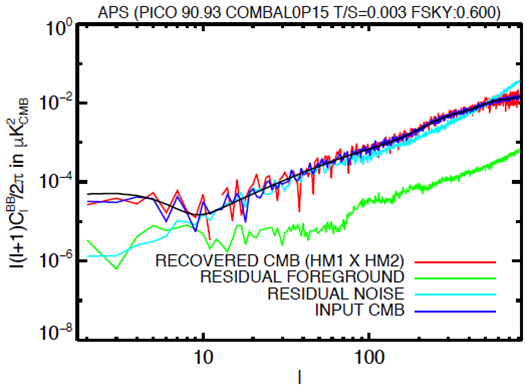
\includegraphics[width=3.0in]{images/soumen_NILC_foregrounds_93.png}}}
\hspace{0.25in}
\parbox{3.0in}{
\caption{Caption . . . \dotfill
\label{fig:nilc}}}
\vspace{-0.1in}
\end{figure}

%\begin{figure}
%\hspace{-0.1in}
%\parbox{4.0in}{\centerline {
%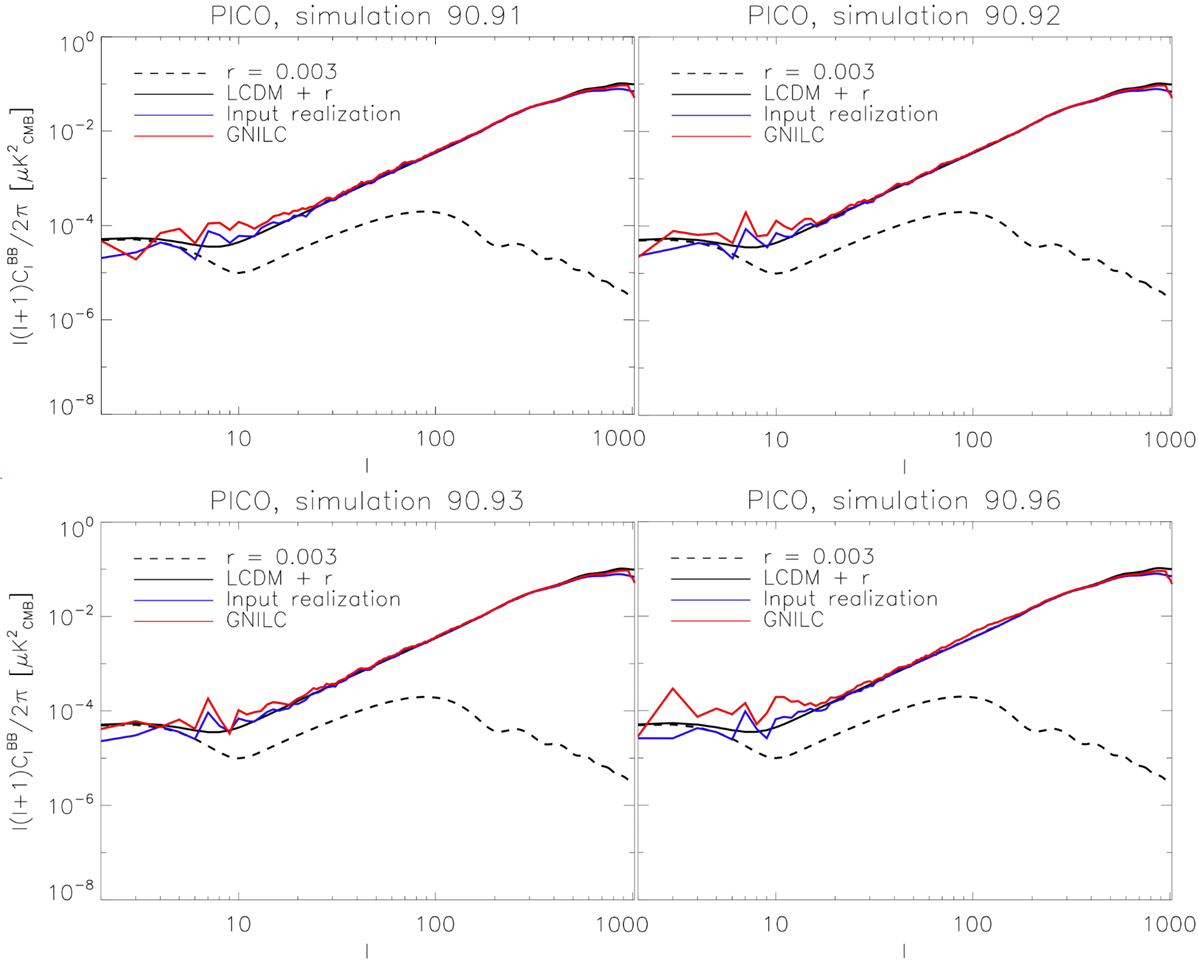
\includegraphics[width=0.6\textwidth]{images/mathieu_GNILC_foregrounds.png}}}
%\hspace{0.in}
%\parbox{2.0in}{
%\caption{Caption . . . 
%\label{fig:gnilc} } }
%\vspace{-0.1in}
%\end{figure}

\begin{figure}
\hspace{-0.1in}
\parbox{4.5in}{\centerline {
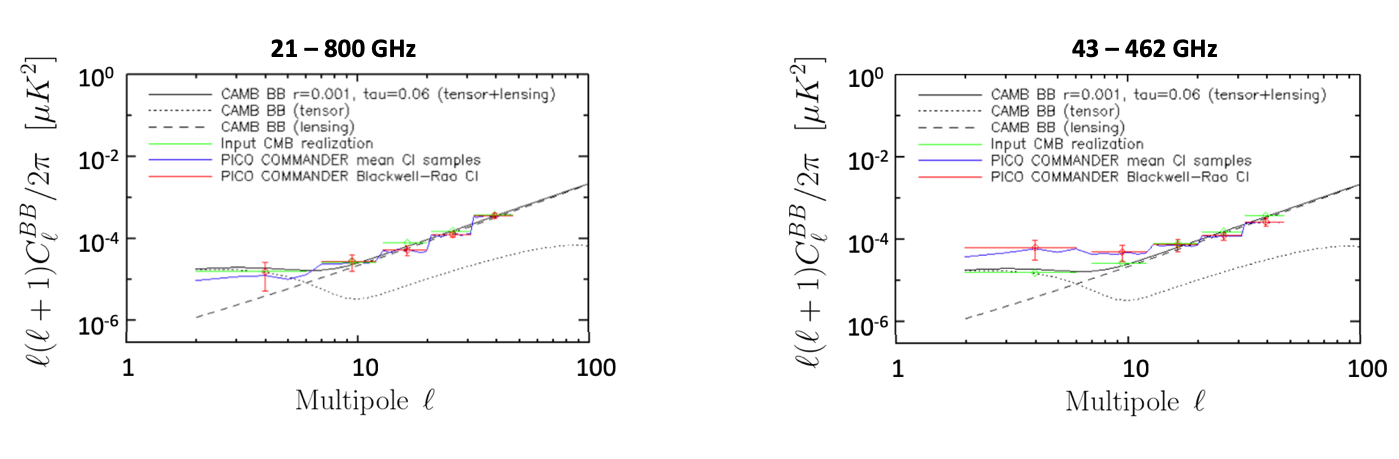
\includegraphics[width=4.5in]{images/commander_foregrounds_BB.png}}}
\hspace{0.in}
\parbox{2.0in}{
\caption{Caption . . .  \dotfill
\label{fig:commander}}}
\vspace{-0.1in}
\end{figure}

The most important lesson arising from our exercise is that more work is required to ascertain that levels of $r \lesssim 0.001$ can be determined robustly on the largest angular scales, that is from the reionization peak.  Figure~\ref{fig:nilc} shows results from the NILC analysis. For several of the sky models the power spectra of the residual level of foregrounds -- that is the level of foregrounds remaining in the map after foreground separation -- is below the cosmological \ac{IGW} level with $r =0.003$. For a minority of the models, the residual is higher at $\ell \lesssim 20$. Results from GNILC, shown in Figure~\ref{fig:gnilc}, are similar. In all cases, the analyses are carried out using 60\% of the sky, the results shown are from one realization, and that no further optimization of the basic foreground separation technique has yet been applied. 

More work is also required to understand the necessary span of frequencies required. Figure~\ref{fig:psm_mr} shows that removing several of PICO's frequency bands, in this case the three highest, significantly biases the extracted $BB$ power spectrum, particularly at the lowest $\ell$ values. This result should not be interpreted as conclusively demonstrating that a frequency span up to 800 GHz has been proven to be essential. At this point of time, different input sky models, coupled to different foreground separation techniques may yield different results. Rather, the conclusion is that further improvement in our modeling and analysis is required. 

While these initial results are encouraging, as they suggest that PICO's frequency coverage and sensitivity may be adequate for this level of $r$, more work should be invested to gain complete confidence that this and lower levels of $r$ can be extracted. This work includes, but not limited to: running more realizations; is ahead to 

Reducing the sky area used to 50 or




\noindent{\bf Required Frequency Span} \hspace{0.1in}


%%%%%%%%%%%%%%%%%%%%%%%%%%%%%%%%%%%
\subsubsection{Discussion}
%%%%%%%%%%%%%%%%%%%%%%%%%%%%%%%%%%%


\end{document}

%\begin{figure}[!htb]
%\centering
%
\includegraphics[width=4cm]{images/example}
%\caption{example}
%\label{fig:im_3}
%\end{figure}


%The baseline design of PICO has 21 channels observing the sky in the 20\,GHz to 800\,GHz frequency range (Fig.~\ref{fig:pico-channels-and-fg}). By analysing how the total emission varies across frequency bands, one can infer the detailed emission properties of the various emission components, form linear combinations of the observations that maximise the contribution of a component of interest while minimising contamination by the others and by instrumental noise, and understand the properties of the foregrounds to evaluate potential residuals in the CMB B-mode map. Various such techniques have been successfully used in previous CMB observations such as those of the Planck mission. Building on this existing expertise, we have carried out map based simulations within a ``data challenge'' framework to assess the capacity of PICO to measure the main signal of interest (CMB primordial B-modes). In this process one group prepares sets of simulated maps for different models of foreground emission of varying complexity from optimistic to pessimistic, which are placed in a shared area. These are then re-analyzed by multiple individuals and groups employing various different component separation algorithms.

